\documentclass[10pt,a4paper]{article}
\usepackage{clrscode}
\usepackage[conEntregas]{caratulaTP1}
\usepackage[spanish]{babel} % para que comandos como \today den el resultado en castellano
\usepackage{a4wide} % márgenes un poco más anchos que lo usual
\usepackage[T1]{fontenc}
\usepackage{textcomp}
\usepackage{graphicx}
\usepackage[utf8]{inputenc} 
\usepackage{pdfpages}
\usepackage{xcolor}
\usepackage{amsmath}
\usepackage{ftnxtra}
\begin{document}



\titulo{Trabajo Práctico 1}
\subtitulo{Eligiendo justito}

\fecha{\today}

\materia{Algoritmos y Estructura de Datos III}

\integrante{Buceta, Diego}{001/01}{diegobuceta35@gmail.com}
% Pongan cuantos integrantes quieran

\maketitle

\newpage
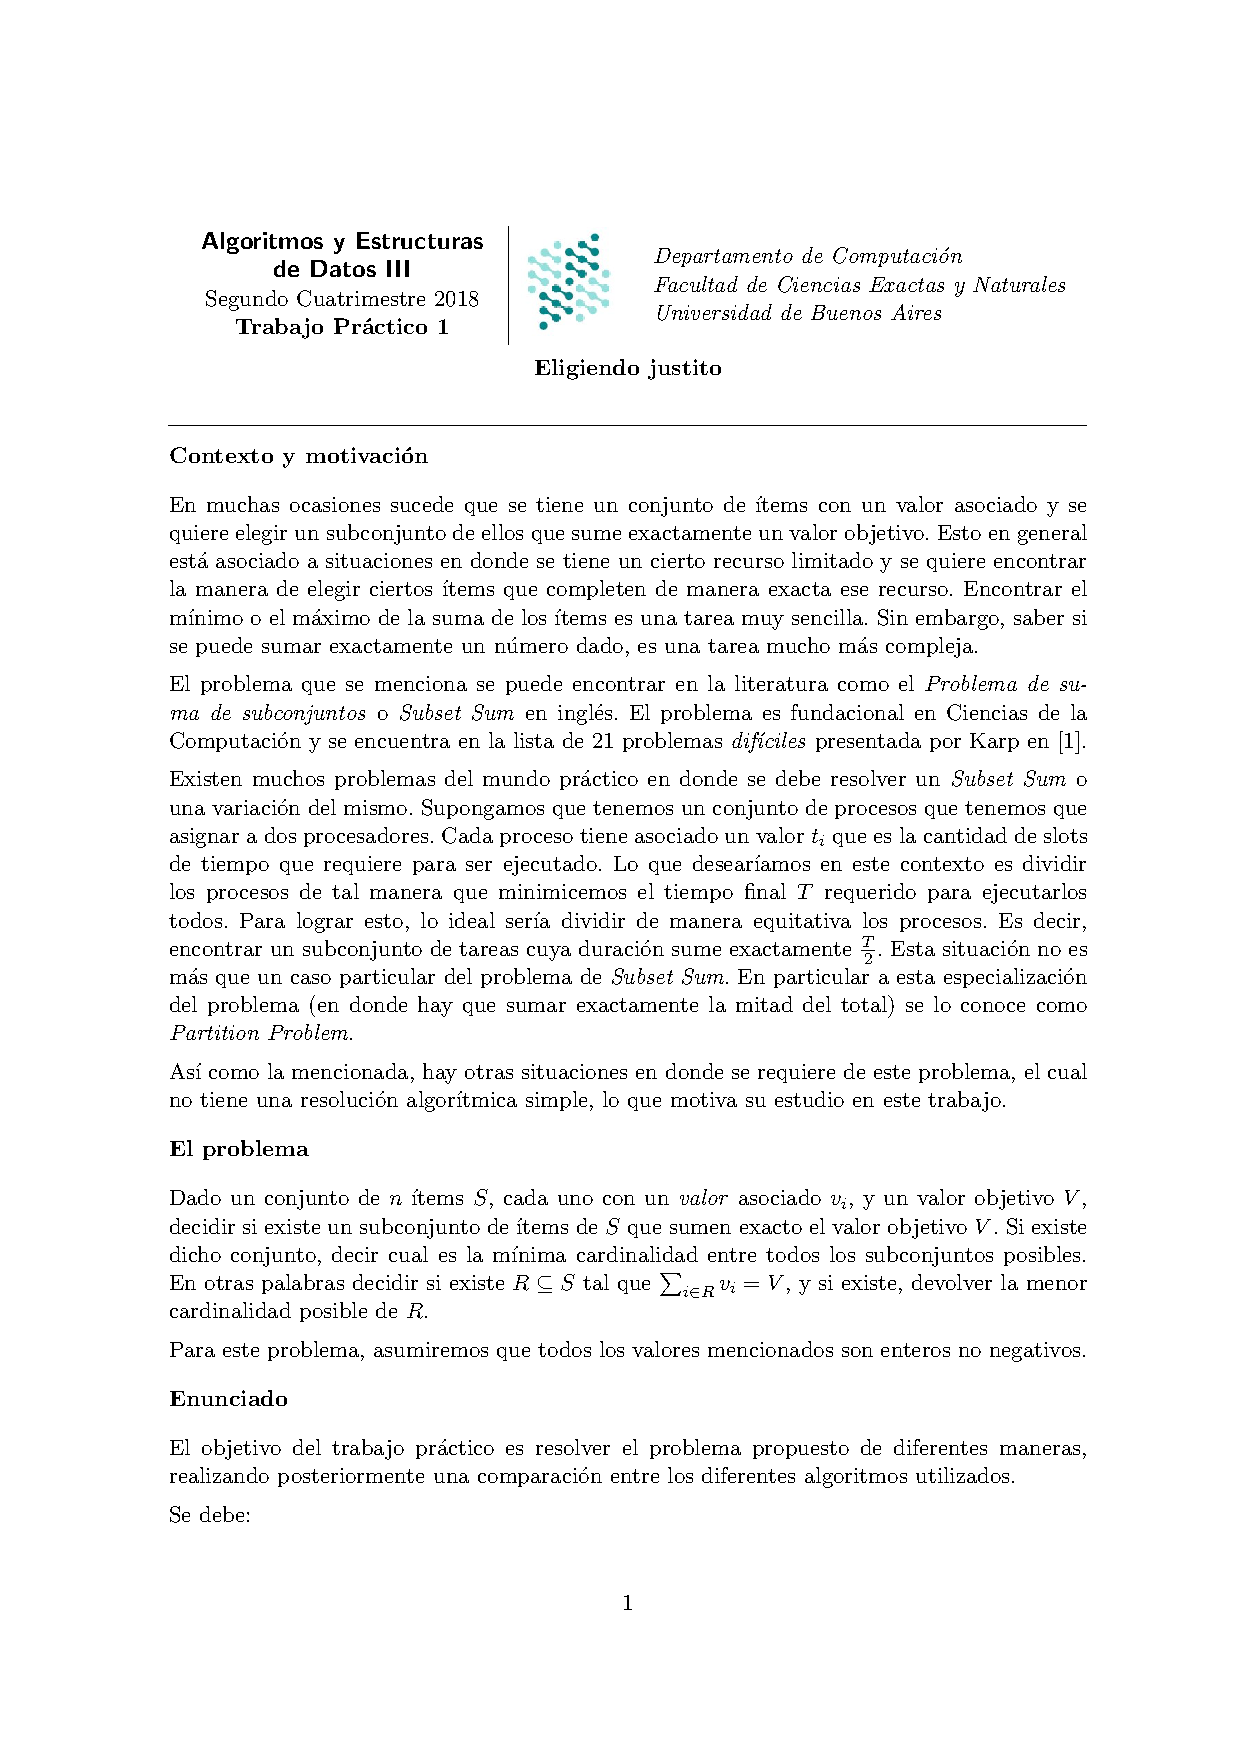
\includepdf[pages={1,2}]{tp1.pdf}

\section{El problema}
	

\newpage
\section{Técnica de Fuerza Bruta}
\bigskip
Esta forma de resolver el problema consiste en definir un dominio de posibles soluciones del problema que consideremos y un algoritmo que permita alcanzarlas a todas. 

\bigskip

	En nuestro problema, vamos a definir nuestro espectro de posibles soluciones al conjunto de partes del conjunto inicial, S. Este conjunto estará formado por todos los posibles subconjuntos que se puedan tomar con elementos de S. Dado que cada elemento tiene dos opciones, estar o no en un determinado subconjunto, las opciones entonces son:
	\[2 \cdot 2 \cdot 2 \cdots 2 = 2^{n} \]	
Por la propia definición, es trivial que si llegará a existir un conjunto R contenido en S y que la sumatoria de sus elementos sea V lo vamos a poder encontrar. Además, almacenando como nueva solución sí y solo sí la encontrada es mejor que la anterior o si no existía,se encontraría en particular la que tenga menos elementos.

\bigskip
\subsection{Complejidad}
Desde el punto de vista de complejidad, la definimos en función del tamaño de entrada, y tomando n como el tamaño de S, nuestro algoritmo será $\theta$(n $\cdot$ 2$^{n}$), porque se recorrerá cada subconjunto del conjunto de partes de S y para cada uno revisaríamos cuáles de los n elementos de S están en ese subconjunto.

\bigskip


\bigskip
\section{Backtracking}
En esta técnica también es necesario definir el espectro de posibles soluciones del problema. Vamos a considerar también que éstas son el conjunto de partes de S.
Lo que caracteriza a esta forma de resolver el problema es que vamos a buscar definir situaciones en las que seguir computando la solución no tenga sentido. A esto se lo llama podas y existen de dos tipos: por optimalidad y factibilidad. Dado que en nuestro problema vamos a operar con los elementos de todos los posibles subconjuntos de S, es razonable imaginar que muchas operaciones se realizarán múltiples veces. 

Para formar el subconjunto solución se recorrerán los n elementos de S. Sea un subconjunto vacío R, se fijará en la primera posición cada uno de los valores de S y para los siguientes posiciones de R, n, se aplicará recursivamente nuestro algoritmo con \[ S' = S - \{e_{1}\} \] Nuestras podas estarán determinadas por lo siguiente:

\subsection{Podas}
\begin{itemize}
	\item 
	Por optimalidad: Si en el proceso de computo de una posible solución, se llegará al caso en que el subconjunto de elementos actual contiene más elementos que la mejor solución encontrada hasta ahora, entonces no se buscará y computará ninguno de los subconjuntos que surjan de tener como los primeros k elementos del subconjunto actual y siendo k el tamaño de éste. A nivel algorítmico significará que esa a partir de esa posición no se buscará las posibles combinaciones con los elementos restantes de S’.
	
	\item 
	Por factibilidad: Si en el proceso de cómputo de una posible solución, se llegara al caso en que la sumatoria de los elementos del conjunto formado actual supera a V, entonces de no buscarán los conjuntos que surjan de combinar los elementos restantes de S con el conjunto actual.
\end{itemize}



\bigskip

La siguiente imagen muestra la idea de las podas. Si tomamos el punto amarillo superior como el inicio de una parte de los posibles caminos del problema total vemos cómo las flechas verdes marcan los caminos que se siguieron por cada nodo y cómo al llegar a puntos \textcolor{red}{problemáticos} las flechas rojas marcan el retroceso y recorrido de otro camino, hasta agotarlos a todos. Los puntos \textcolor{red}{problemáticos} simbolizan otros inicios de conjuntos de caminos que por algún motivo se decide 'podarlos' y no analizarlos en profundidad.

\begin{center}
\includegraphics[scale=.4]{backtrack}
\footnote{Imagen tomada del blog de Steve Pemberton}
\end{center}


En las podas de factibilidad, buscamos caracterizar cómo es un subconjunto que no puede ser solución y dejar de computar todos los demás ‘subconjuntos padre’, es decir, los que contengan a éste. Por otro lado, para una cota optimalidad se identificará las situaciones en las que seguir computando un subconjunto no tenga sentido debido a que en el mejor caso, es decir, si llegara a ser solución, no sería mejor que la que ya encontramos.


\bigskip

\subsection{Complejidad}

Respecto a la complejidad algorítmica y dado que la establecemos en función de tamaño de la entrada, $|$S$|$ y V, y para el peor caso, también tendrá complejidad asintótica perteneciente a O(n $\cdot$ 2 $^{n}$).\\
El peor caso sería un valor objetivo mayor que la sumatoria de todos los elementos de S. En ese caso nunca se utilizarán ninguna de las dos podas y se llegarán a formar las 2$^{n}$ combinaciones de conjuntos, con sus respectivos cómputos de sumas interiores.\\ \\
Analicemos algunos puntos de diferencia y similitud entre los algoritmos
\begin{itemize}
	\item En fuerza bruta la complejidad es la teórica en el mejor y peor caso, es decir, $\in$ $\theta$(n $\cdot$ 2 $^{n}$) porque siempre se analizará todas las posibles soluciones del dominio definido inicialmente.


	\item En backtracking la cota superior $\in$ O(2$^{n}$ $\cdot$ n), pero su cota inferior no es la misma. Por ejemplo, si todos los elementos de S superan a V, entonces la cantidad de pasos realizada sería O($|$S$|$), dado que al poner el primer elemento entraría la poda de factibilidad y se descartarían todos los subconjuntos con el $e_1$ dentro y se agregaría el siguiente. Como ninguno los elementos de S puede estar en el conjunto solución, esto se repetirá hasta que no queden elementos por agregar, iterando sólo |S| veces.
	
\end{itemize}

\section{Programación Dinámica}

Esta técnica se basa en utilizar la metodología de {\it divide and conquer \footnote{Metodología que busca simplificar un problema grande o complicado en problemas más chicos y simples de una forma recursiva}} y almacenar los resultados calculados para no tener que volver a hacerlo cuando se repita un problema. Para poder aplicar usar programación dinámica es necesario que se cumpla entonces: 
\begin{itemize}
	\item
	El problema pueda ser dividido en subproblemas y que la solución que se encuentre para cada uno de ellos sea óptima, para así construir la solución del problema inicial de forma óptima \footnote{Este concepto suele denominarse como: {\it principio del óptimo}}
	
	\item 	
	Los subproblemas compartan soluciones\footnote{Se denomina a esto subproblemas superpuestos y un ejemplo muy conocido es la sucesión de Fibonacci}
\end{itemize}



\bigskip

AGREGAR EXPLICACION DEL ANALISIS PARA LLEGA
Se define PD una función que recibe un conjunto S, de elementos enteros mayores a 0 y un valor V entero mayor a 0, y devuelve el mínimo cardinal del subconjunto s perteneciente a S que todos los elementos suman V; si no existe se devuelve infinito. \\
\[
\begin{array}{@{} r @{} c @{} l @{} }
&PD(S, V) = PD($\{$e_{1},e_{2},\dots,e_{n}$\}$,V) &{}=\displaystyle
\begin{cases}
\ \infty &\text{si } \text |S| = 0 \wedge V \neq 0 
\\
\ 0 &\text{si } \text V = 0 
\\
PD($\{$e_{2},e_{3},\dots,e_{n}$\}$,V)  &\text{si } e_{1} $>$ V
\\
\min_{} (1 + PD($\{$e_{2},e_{3},\dots,e_{n}$\}$,V - e_{1}),PD($\{$e_{2},e_{3},\dots,e_{n}$\}$,V))&\text{otro caso }
\\
\end{cases}
\end{array}
\]
\end{document}
